\section{Chamber Production}
	
	\subsection{Construction Process}
		\begin{frame}{High Bay}
			
		\end{frame}
		\begin{frame}
			\scalebox{0.65}{
				\begin{minipage}{0.5\pdfpagewidth}
							\begin{description}
							\item [Week 1:] \colorbox{googlegreen}{Tube Gluing}
								\begin{itemize}\small
									\item Glue 2 layers per day (including gluing spacer frame/RASNIK layer)
								\end{itemize}
							\item [Week 2:] \colorbox{googlegreen}{Position Measurements}
								\begin{itemize}\small
									\item Measure wire heights 
									\item Glue AP-plates, B-field sensors, CCC platforms.
									\item Measure platforms.
									\item Glue support bars.
								\end{itemize}
							\item [Week 3:] \colorbox{googleblue}{Gas Systems}
							\item [Week 4:] \colorbox{googleyellow}{Cosmic Ray Test}
						\end{description}
					\end{minipage}
					}
			\hfill
			\begin{minipage}{0.4\pdfpagewidth}
				\begin{figure}
					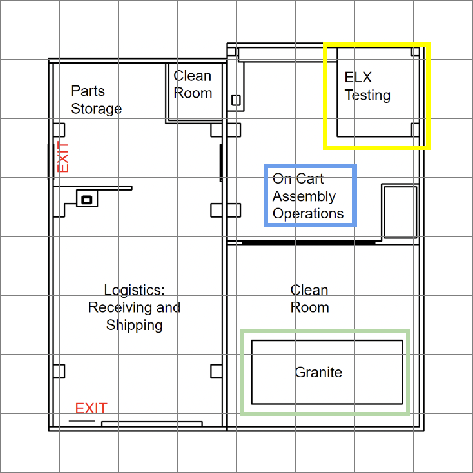
\includegraphics[width=0.4\pdfpagewidth]{test.pdf}
				\end{figure}
			\end{minipage}
		\end{frame}
		\begin{frame}{\ph}
			\begin{figure}[t]
				\centering
				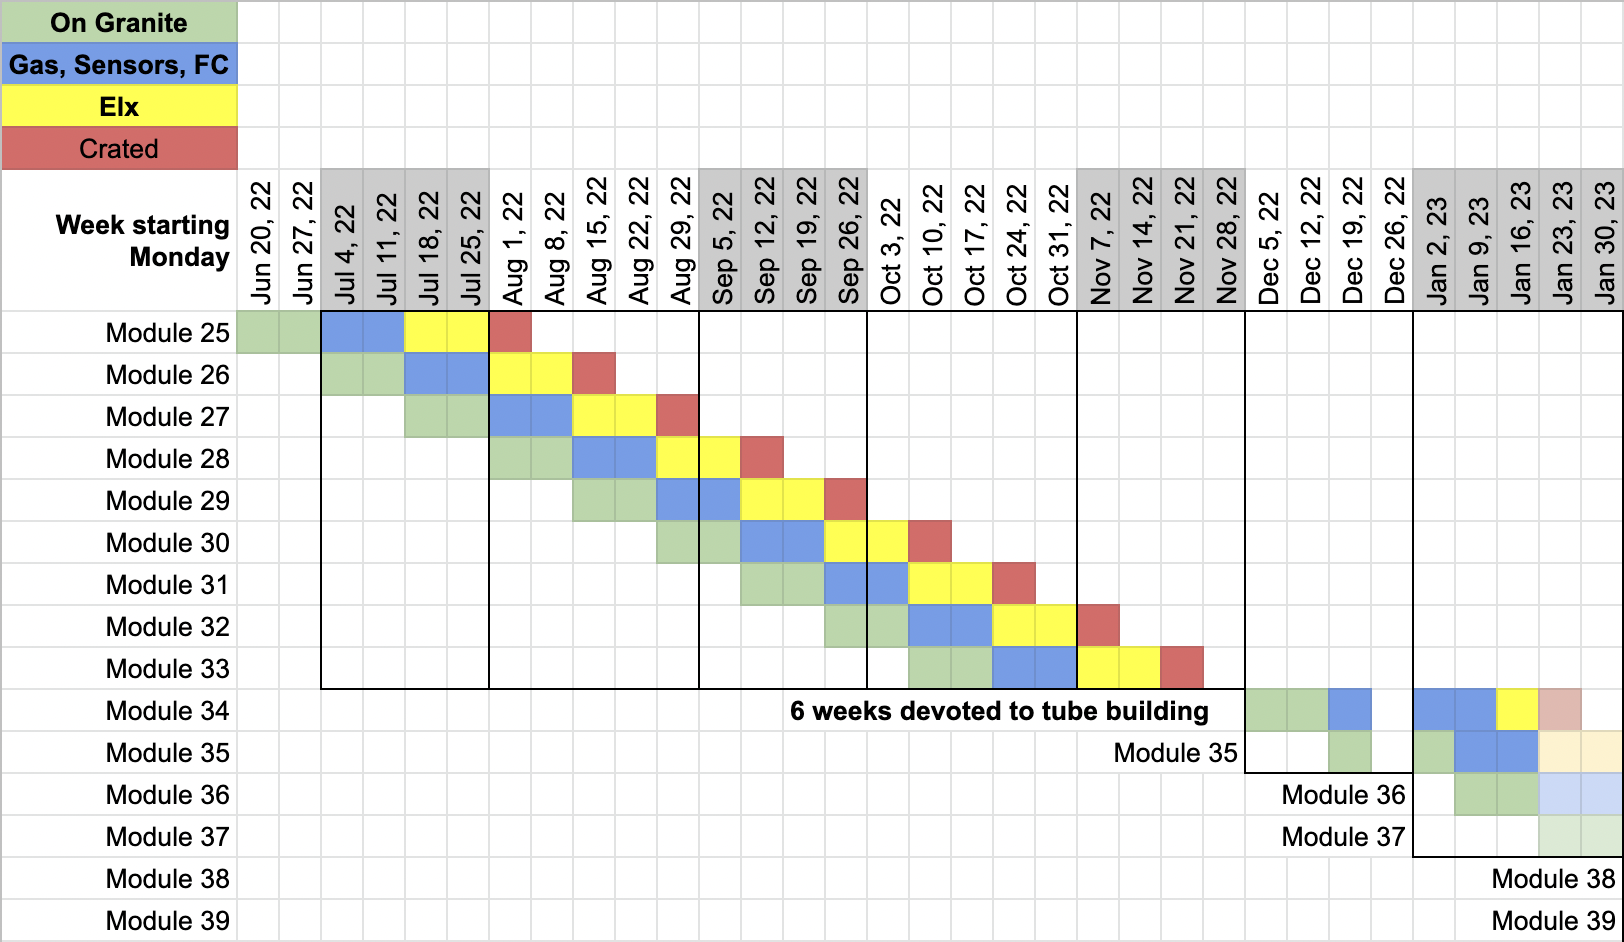
\includegraphics[width=0.8\pdfpagewidth]{Chamber Production.png}		
				\label{fig:ChamberProduction}		
			\end{figure}
		\end{frame}
	\subsection{Testing}

		\begin{frame}{Measurements \ph}
			\begin{itemize}
				\item Platform positioning
				\item Endplug height positioning (different from mpi)
				\item we domt have coordinate measuee machine, measure endplug height, assume z direction is fine, set by combs
				\item layer spacing layer pitch
				\item Leak Rate
				\item Effeciency
				\item Resolution
			\end{itemize}
		\end{frame}
		\begin{frame}{Wire Height \ph}
			\begin{figure}
				\centering
				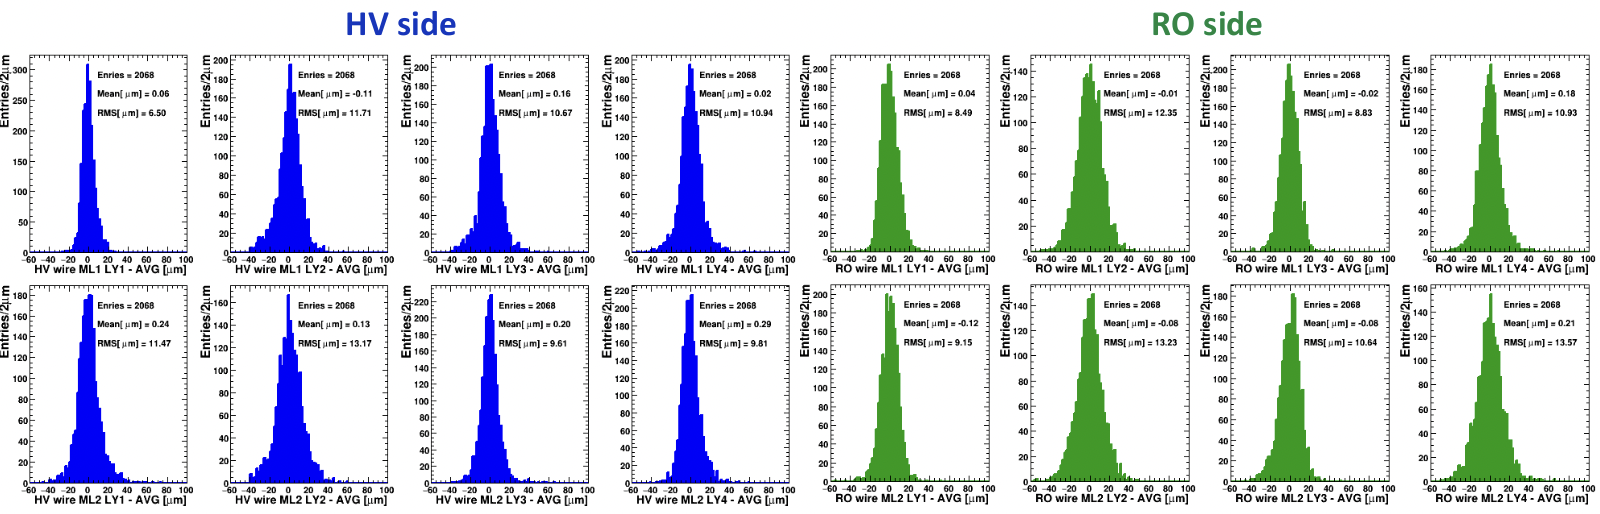
\includegraphics[width=0.6\pdfpagewidth]{WireHeightOffset.png}
			\end{figure}
		\end{frame}
		\begin{frame}{Inplane Alignment \ph}
			\framebox{\begin{figure}
				\begin{subfigure}[c]{0.3\pdfpagewidth}
					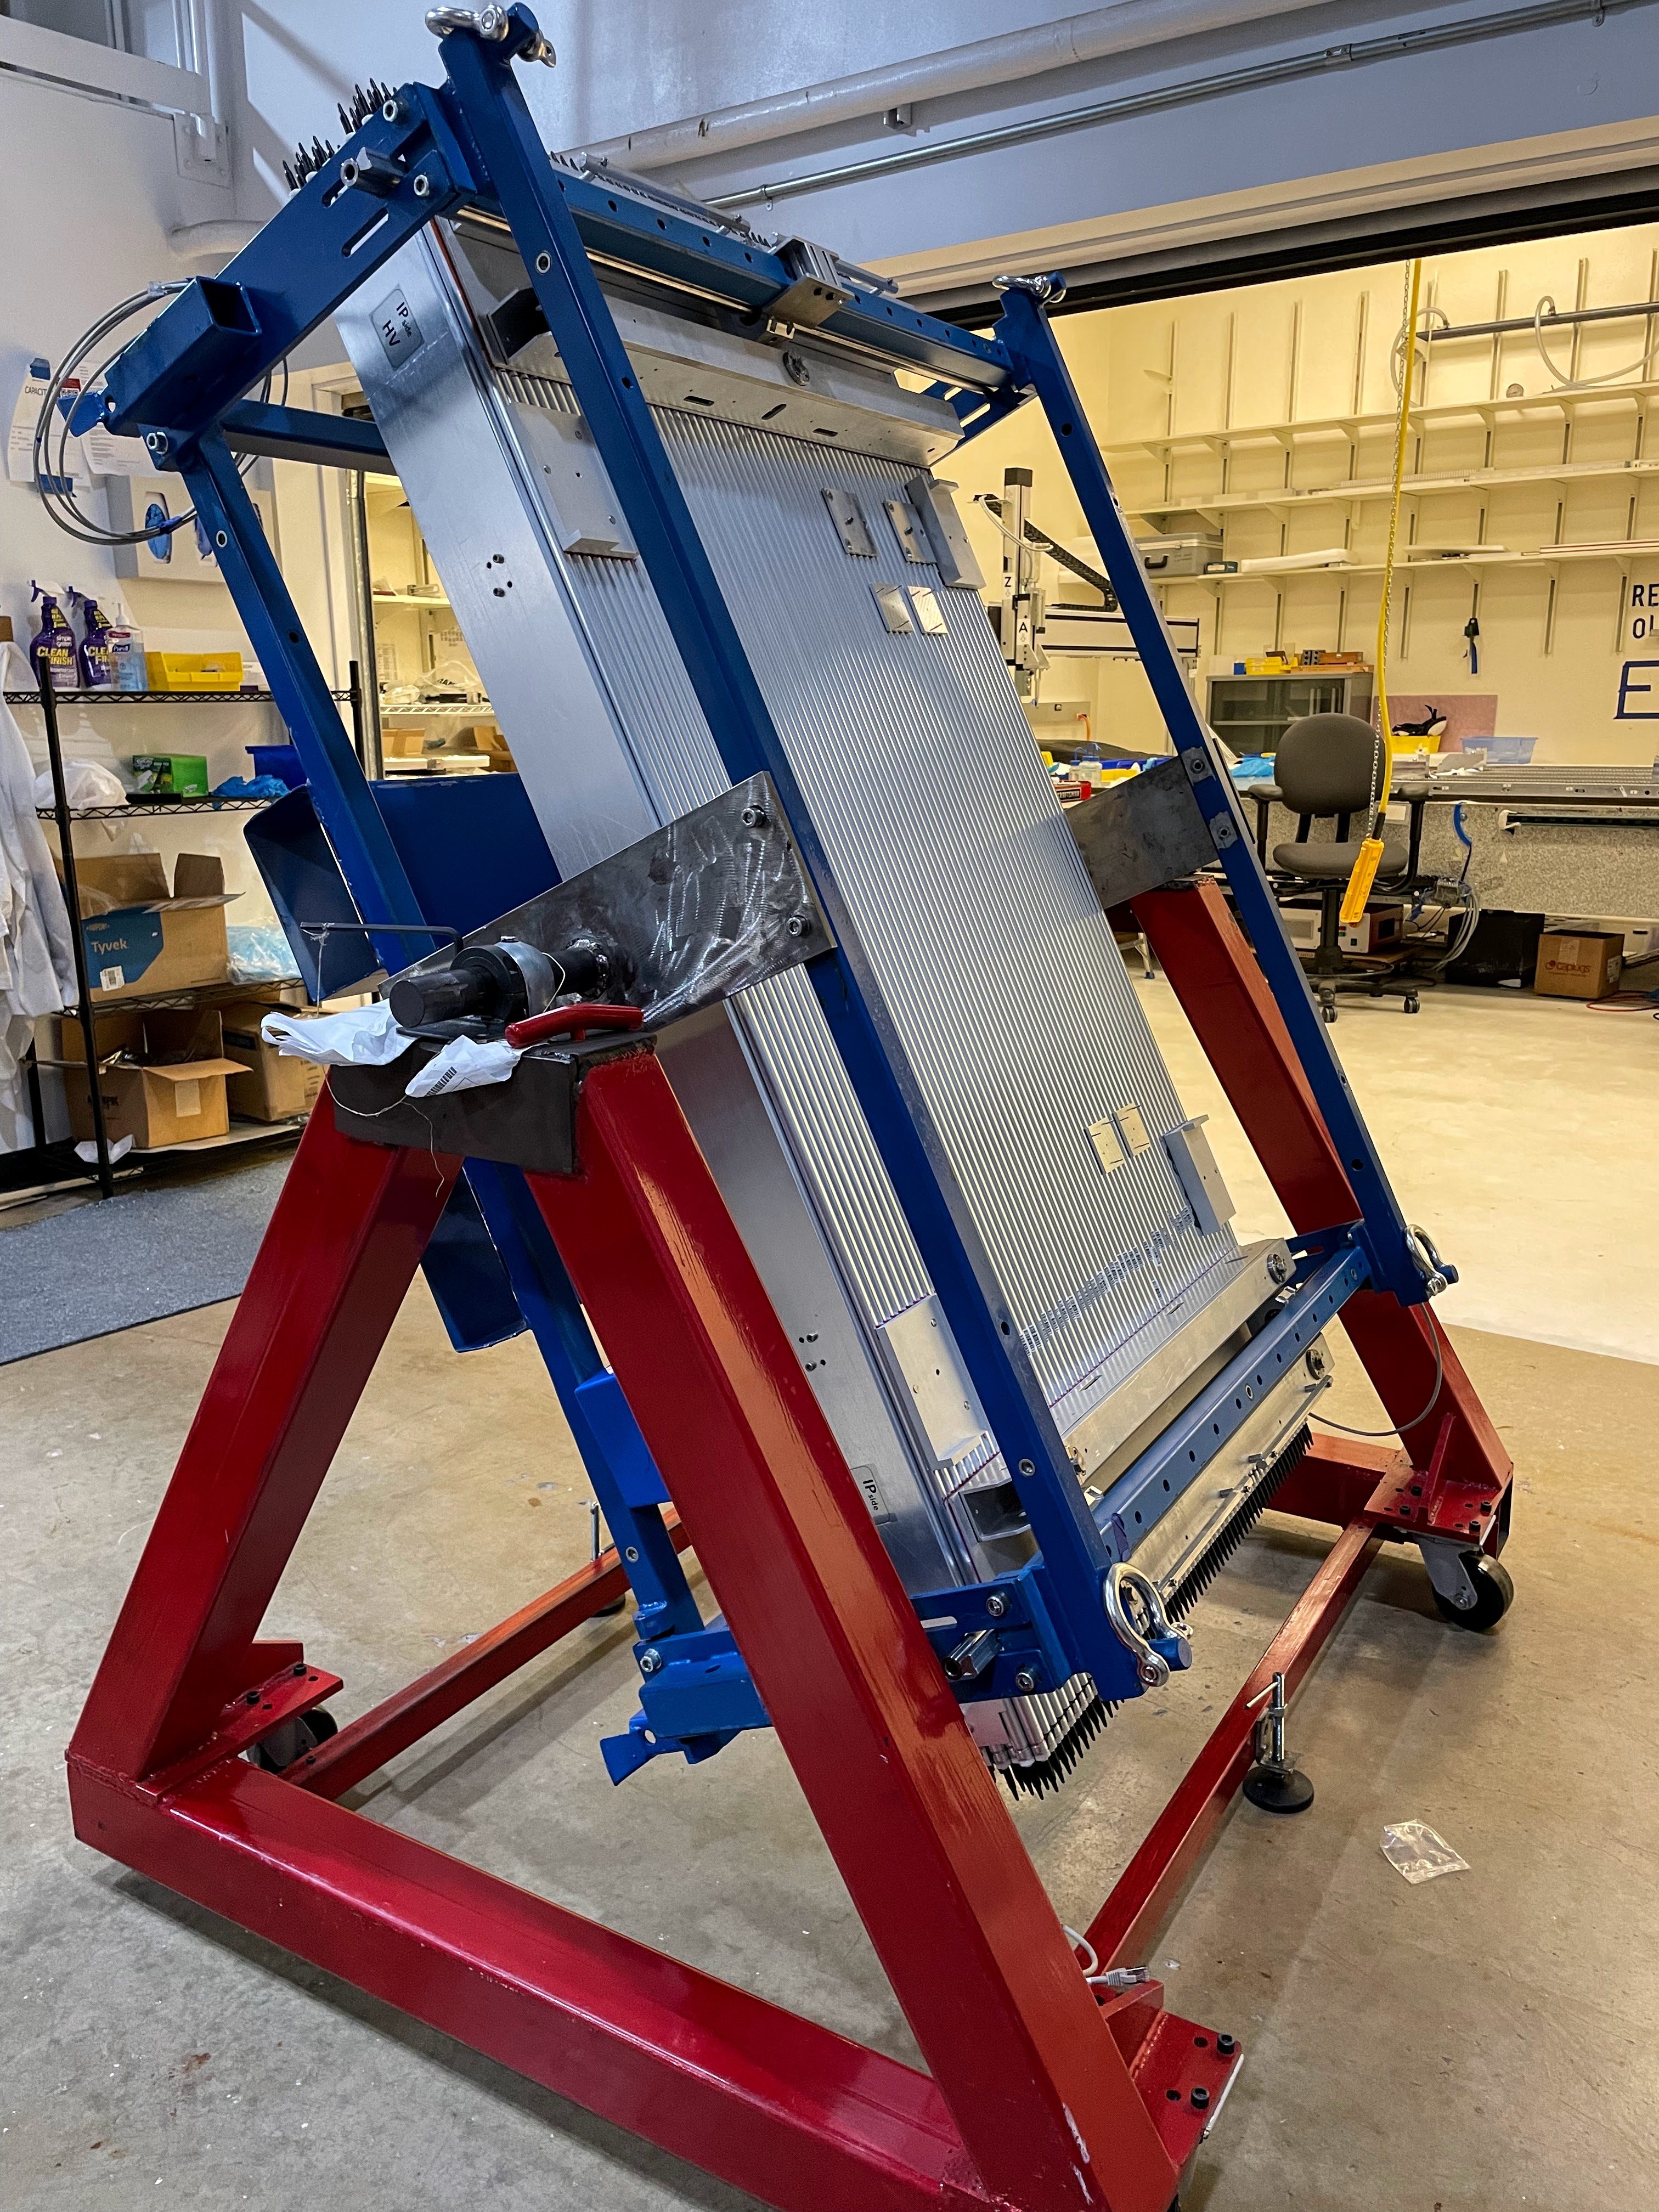
\includegraphics[height=0.4\pdfpageheight]{RotationCart.jpg}
					\caption{Chamber on rotation cart}
					\label{fig:RotationCart}
				\end{subfigure}
				~
				\begin{subfigure}[c]{0.5\pdfpagewidth}
					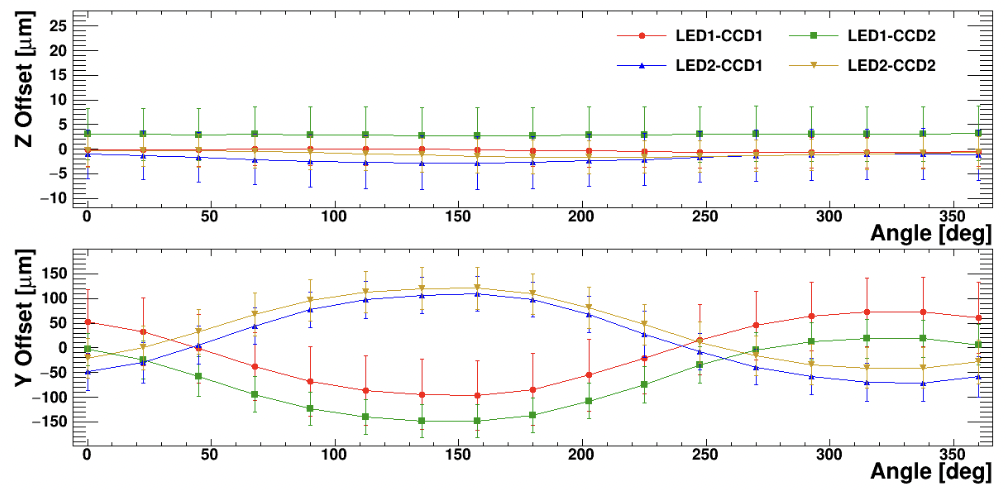
\includegraphics[width=0.4\pdfpagewidth]{RASNIKMeasurements.png}
					\caption{Deviation}
					\label{fig:InplaneAlignment}
				\end{subfigure}
			\end{figure}}
		\end{frame}

		\begin{frame}{Leak Rate \ph}
			\begin{figure}
				\centering	
				\begin{subfigure}[t]{0.4\pdfpagewidth}
					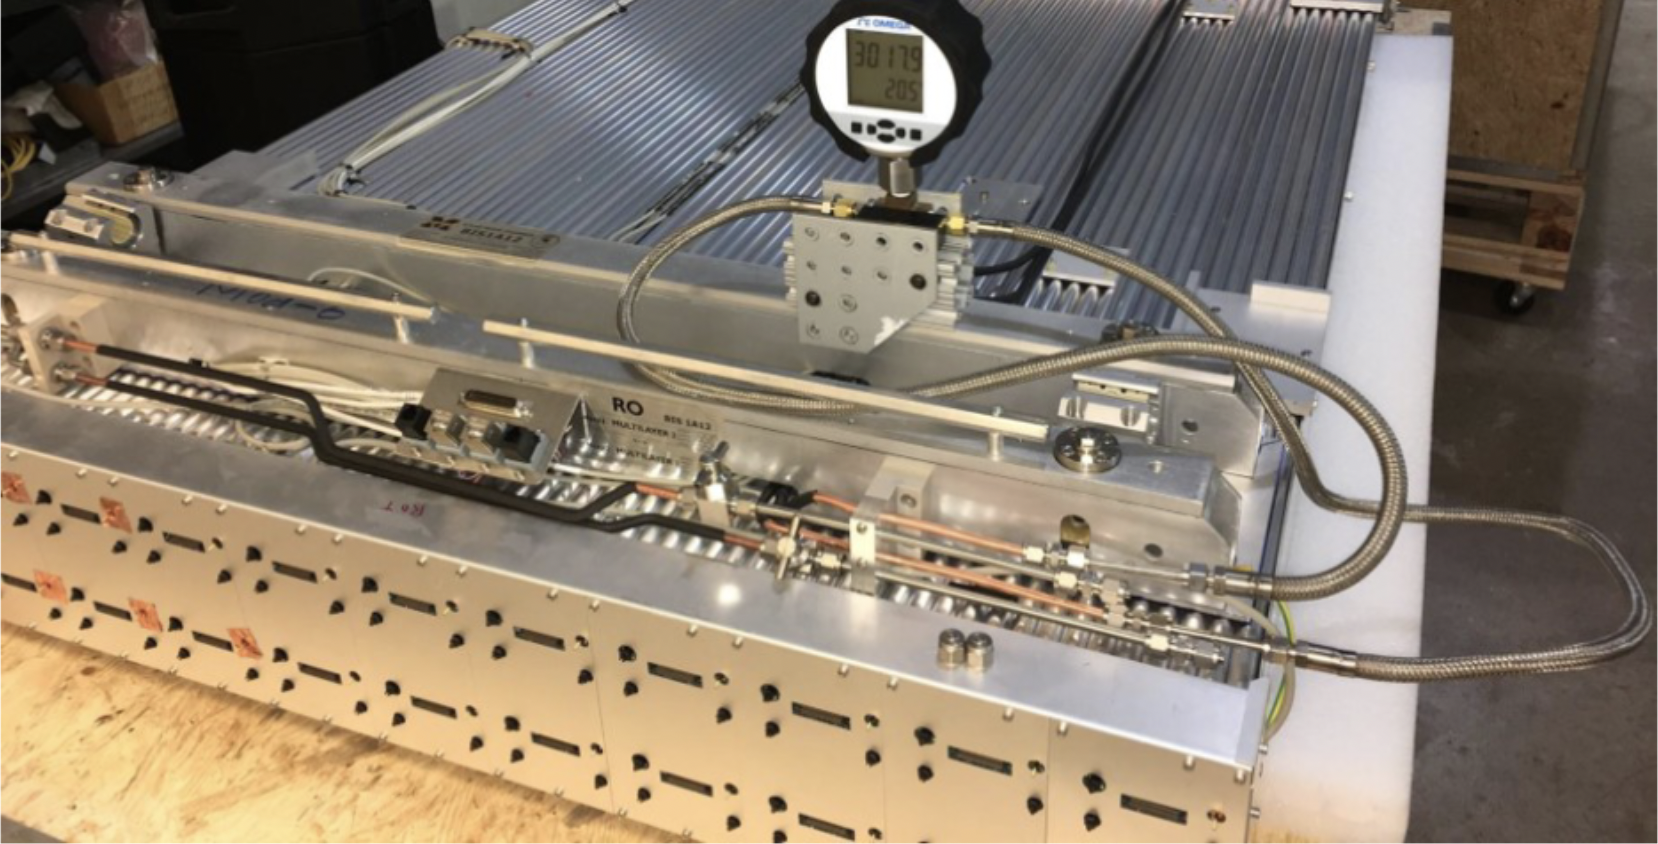
\includegraphics[width=0.4\pdfpagewidth]{PressureGauge.png}
					\caption{Chamber undergoing a pressure drop leak test}
				\end{subfigure}
				\hfill
				\begin{subfigure}[t]{0.4\pdfpagewidth}
					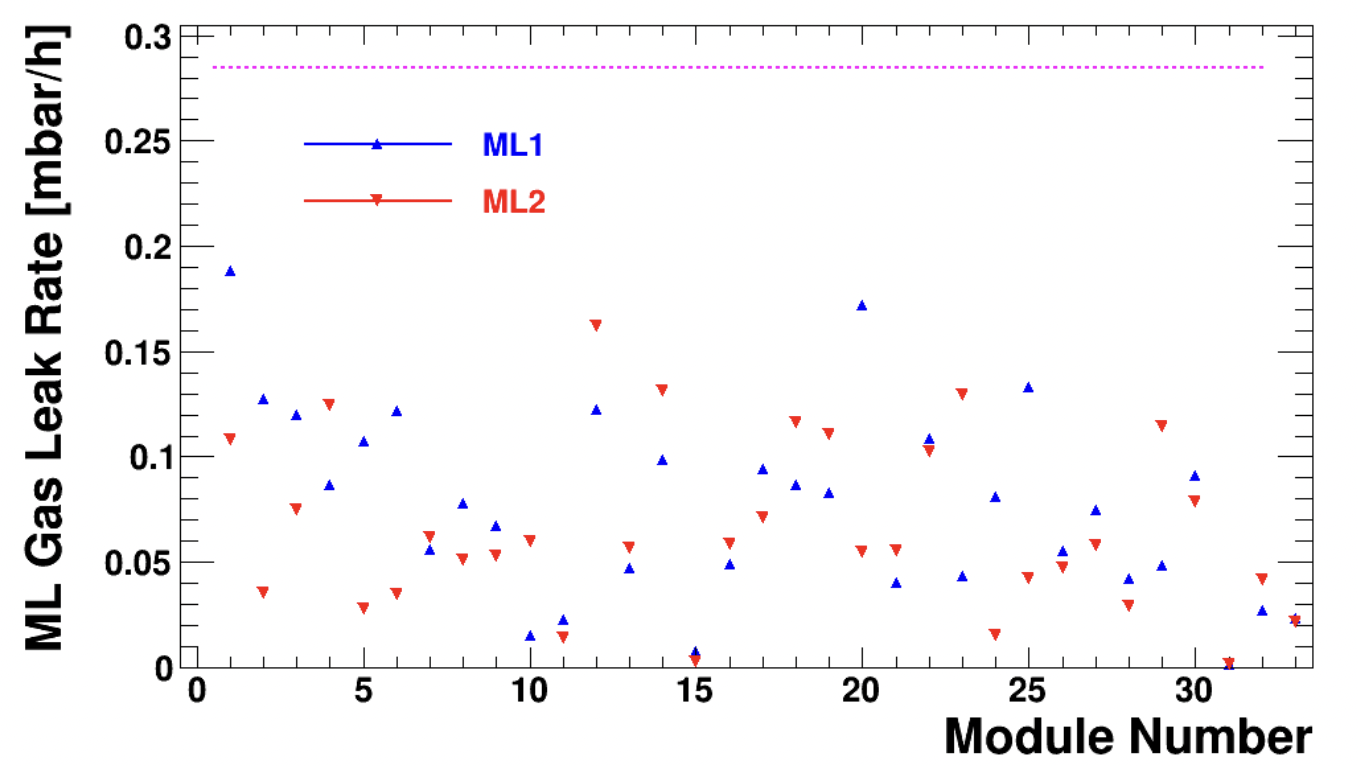
\includegraphics[width=0.4\pdfpagewidth]{ChamberLeakRate.png}
					\caption{Leak Rates of past 35 modules. The dotted pink line is the maximum acceptable leak rate of 0.288 mbar/hr.}
				\end{subfigure}
			\end{figure}
		\end{frame}

		\begin{frame}{Efficiency \ph}
			\begin{figure}[t]
				\centering	
				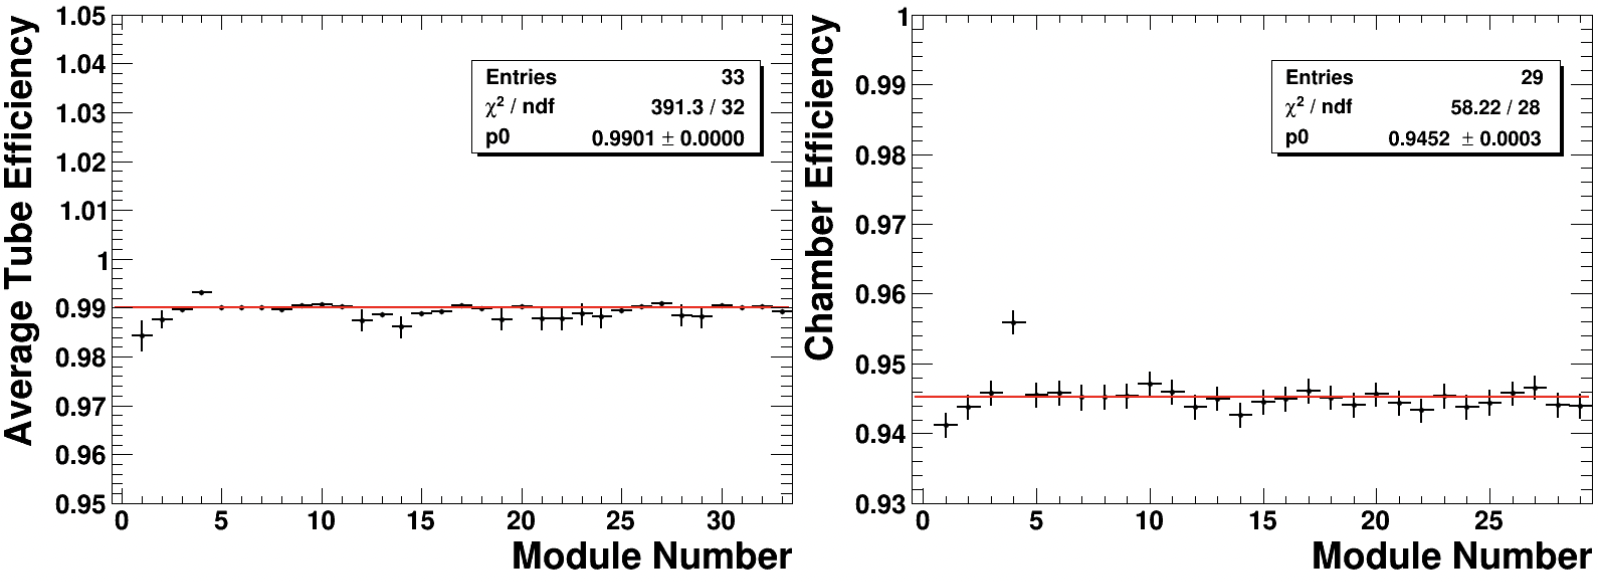
\includegraphics[width=0.8\pdfpagewidth]{ChamberEfficiency.png}
				\label{fig:ChamberEfficiency}
			\end{figure}
		\end{frame}
		
		\begin{frame}{Resolution \ph}
			\begin{figure}
				\centering	
				\begin{subfigure}[c]{0.4\pdfpagewidth}
					\centering
					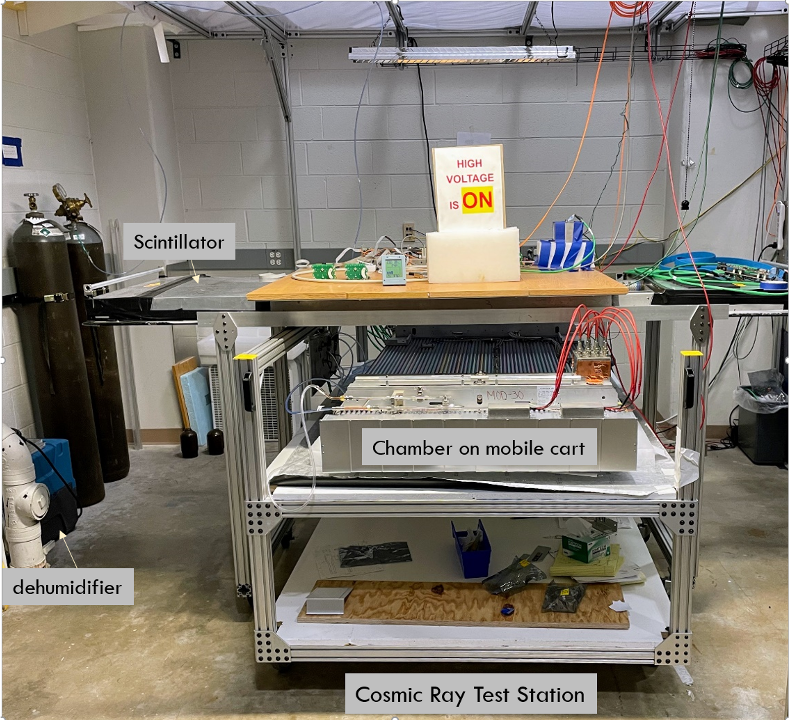
\includegraphics[width=0.3\pdfpagewidth]{CosmicRay-Station.png}
					\caption{Cosmic Ray testing station}
				\end{subfigure}
				\hfill
				\begin{subfigure}[c]{0.4\pdfpagewidth}
					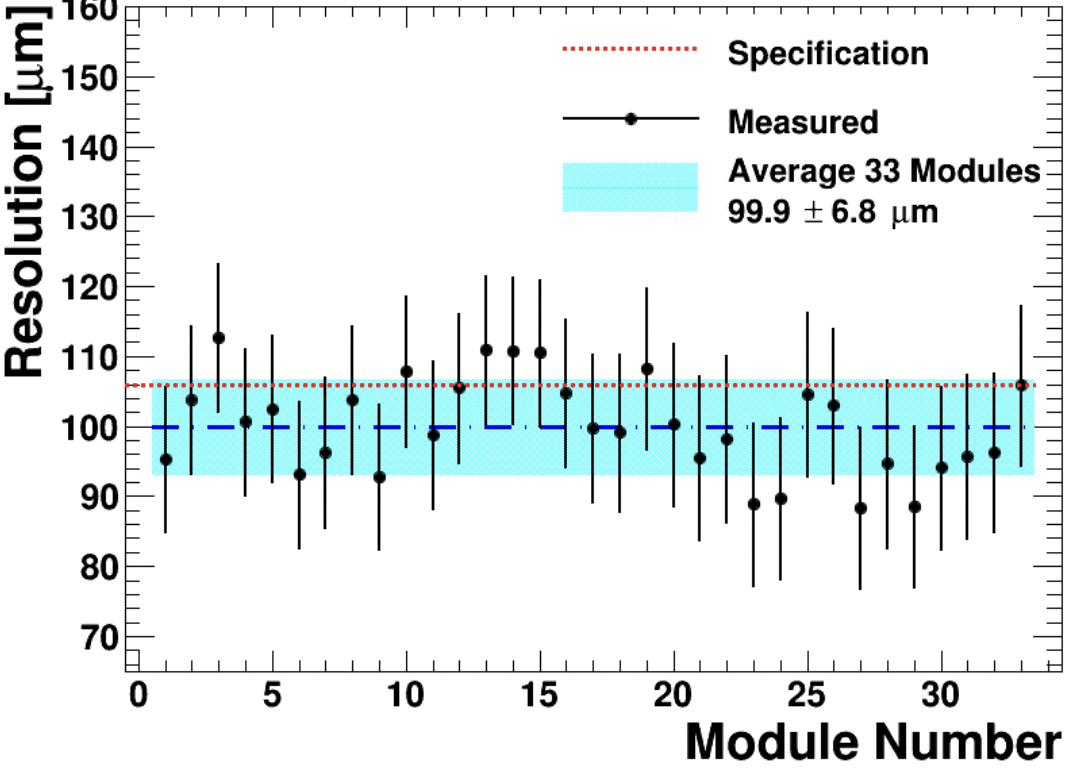
\includegraphics[width=0.4\pdfpagewidth]{ChamberResolution.png}
					\caption{Resolution done with convolutions}
					\label{fig:ChamberResolution}
				\end{subfigure}
			\end{figure}
			mpi takes shorter run, we take out scattering with convolutions
		\end{frame}



	\subsection{Moving Forward}

		\begin{frame}{New Electronics}
			replacing csms (csm catches stuff from mezzanine and sends as light)
			so we neeed new mezzanine cards 
		\end{frame}




